\chapter{Implementation}\label{sec:implementation}
\section {The original tool}
The original tool is a Graphical Integrated Development Environment called QCADesigner, which is both meant for easing the process of layouting a QCA cells based circuit and for simplyfing the process of simulation and collection of the results. The layout view allows to place on the virtual PCB any number of QCA cell and defining if it is an input, output or fixed one. This discrimination makes it possible for the system to understand of which cells it is meaningful to record the polarization (the output cells) and to which one it is meaningful to assign a value (the input cells). Two different ways of simulating the behaviour of the circuit are implemented: the Coherence Vector and the Bistable engines. 

Both the engines realize the abstract notion of Cellular Automata: the status of every cell at a given instant $t$ strictly depends on its state and on that of its neighborhood at $t-1$. The reason why two engines exist is quite simple: Bistable simulates the behaviour of the circuit from a ''logical'' point of view, meaning that it basically ''switches'' the polarization of every cell based on the polarization of the neighborhood and the current clock in \textsl{just one step}. Coherence Vector, instead, calculates at each instant $t$ the current polarization of the cell and that of its neighborhood and integrates over time the differential equations describing this system in order to make it evolve. Their authors compare and contrast these two engines this way: ''...It is believed that although this approximation [that of Bistable engine] is sufficient to verify the logical functionality of a design it cannot be extended to include valid dynamic simulation; but, as a result of its simplicity this simulation engine is able to simulate a large number of cells very rapidly, and therefore provides a good in-process check of the design. For dynamical simulations refer to the coherence vector simulation. ''. A few number of parameters allow for the customization of the behavuor of both engines in order to make the simulation as accurate and fast as possible. A few rules of thumb are available on the web site of the MiNa Group in order to effectively set some of them.

In the original implementation, moreover, it is possible to look at the evolution of the polarization of every cell during the simulation process.
\section {The bottlenecks of the original implementation}
First of all let's make a basic asymptotic analysis of the implementation of the two engines' algorithms: we have $n$ cells that can have an average of $b$ neighbours. The two engines basically runs trough every cell (this goes as $O(n)$) in the design and compute the current polarization based on the polarization of the previous step of all the neighbours (this goes as $O(b)$), and this is done for any possible combination of the inputs (this goes as $O(2^i)$). That is a asymptotic time complexity of $O(2^i*n*b)$  (worst case: $b$=$n-1$) and a space complexity of $O(n)$ (only the vector of the polarizations of every cell must be saved, anything else is computed using these values).

Now, the main bottleneck of the original implementation derives from the \textsl{serialization} of the simulation of a system that could be actually evolved \textsl{in parallel}, both with respect to $i$ (eg: one thread per configuration of the inputs) and with respect to $n$ (eg: one thread per cell per iteration). The original simulation of the system in this serial fashion, moreover, introduces some additive error (even though distributable over all cells randomizing the order in which they are simulated at each iteration) due to an overlapping of the writes related to different time instants. 

Our focus is set, in particular, on the Coherence Vector engine. The evidence of the limitations of the bottlenecks, here, are more evident than in Bistable because there is not not even the stabilization phase that would require additional costly synchronization mechanism/convergence criteria at each iteration of the simulation. This absence makes it simpler and more cost effective (?) the exploitation of a parallel paradigm.

Before starting talking about the improved version it is good to remember that a number of runs of a set of test circuits has been made with QCADesigner in order to establish the baseline for the evaluation of the progresses (measured in seconds necessary to run the entrire simulation).
\section {Parallelization in CUDA}
\subsection{The approach}
The guiding idea during the parallelization process is: any cell in the system evolves independently of the evolution of the other cells at the same time, but only on the previous state of the machine. Moreover, any input configuration is totally independent on every other possible configuration. In line of principle, this could be approached in one (or both) of these two ways:
\begin{itemize}
\item parallelize with respect to $i$: spread the computation of all the possible $2^i$ configuration on that many threads.
\item parallelize with respect to $n$: spread the computation of all the cells belonging to the same iteration on that many threads.
\end{itemize}
Our choice has been to follow the second approach, mainly because 
\begin{itemize}
\item the "one cell-one thread" approach is easy both to figure out and to manage
\item parallelizing with respect to the number of inputs would make the single kernel \textsl{very} complex, disallowing a number of possible optimizations (eg:occupancy improvement, branch divergence)  
\item not the very same actions should be taken for every cell at any moment of the simulation of different inputs; this introduces a hurdle in terms of branch divergence that doesn't allow the gpu to fully exploit its potential
\item suppose to be simulating $k$ configurations of the inputs at a time. The spatial complexity of the algorithm becomes $O(k*n)$ ($k$ systems characterized by $n$ cells). In the second case only the current and the future states must be recorded ($O(2*n)$)
\end{itemize} 

Moreover, the second approach allows us to better exploit the SIMD principle proper of all CUDA enabled devices because inside the same iteration of the simulation the actions to be carried over any cells are quite the same (and those cells who are not complying with this general scheme don't induce particularly critic divergences in the kernel). This approach allows for the same instructions to be concurrently executed on different data. In our particular case, the code basically does the same actions of the original implementation, apart from the details regarding the proper distribution of the computation among the available resources.

Last but not least, no \textsl{tile-problem} exists (the problem of overlapping adjacent concurrently simulated areas of circuit) because every single cell evolves independently of the effects of the neighbours at the \textsl{same} time $t$.

\subsection{The big picture}
Now let's dive a little deeper into the implementation.

\begin{figure}[h!]
	\begin{center}$
		\begin{array}{cc}
			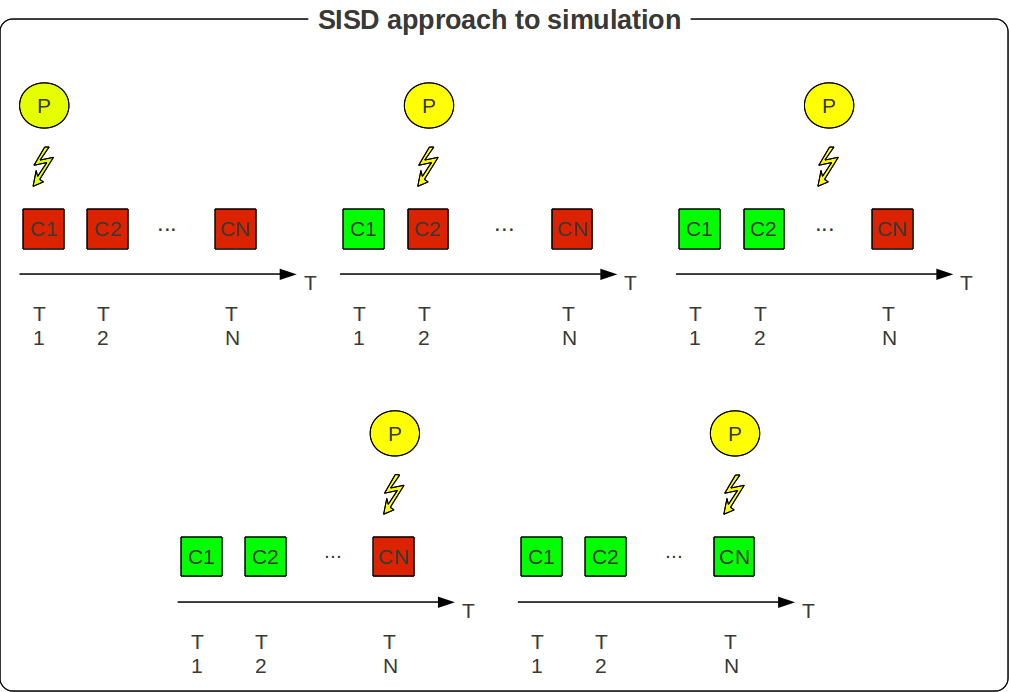
\includegraphics[width=0.5\textwidth]{img/impdetsisd.png} &
			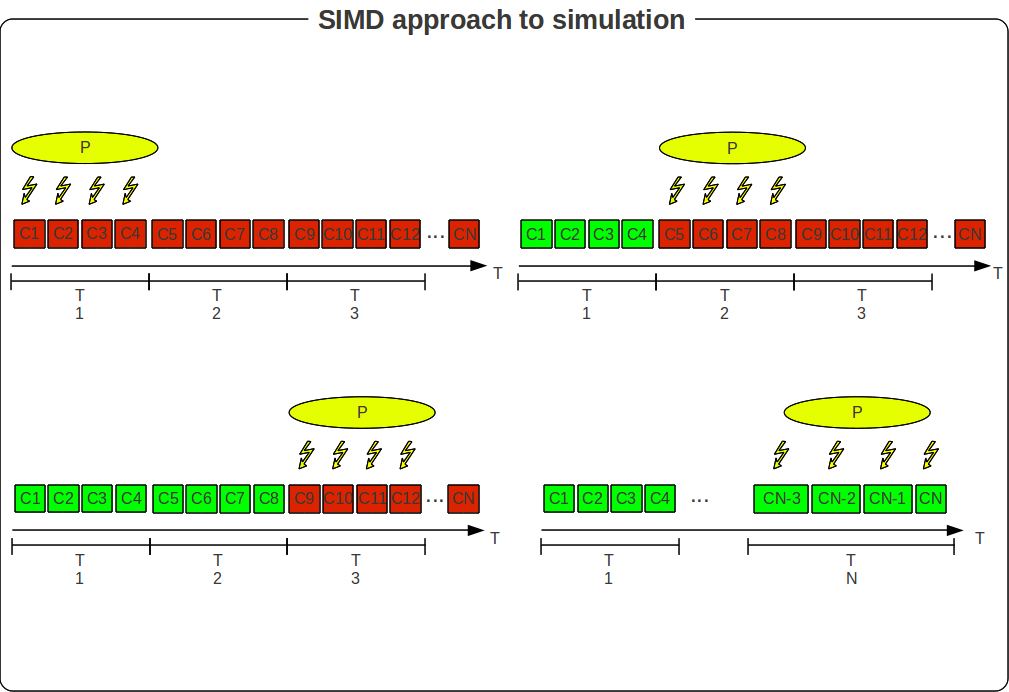
\includegraphics[width=0.5\textwidth]{img/impdetsimd}
		\end{array}$
	\end{center}
	\caption{\label{fig:impdet}In the first approach (SISD) each cell is evolved into the new state \textsl{once at a time}. Observing that any cell inside the same iteration can be evolved \textsl{in parallel} allows us to exploit a SIMD architecture in order to replicate the same instructions over a large number of cells at a time.}
\end{figure}

After an initial phase of parsing the command line commands, the flow of the program goes into Bistable or Coherence Vector engine.

In Coherence Vector mode, three different things happens: first, all the useful data structures are initialized (for the output, for the parameters of the solver, for the iteration over all the cells into the design, notably). Among the others, some structures we had to implement in order to ease the process of converting the orignal data to CUDA compatible ones. In particular, we extract the following data:
\begin{itemize}
\item \textsl{polariztion vector} the vector of the initial polarization of every cell  (size: $n$)
\item \textsl{neighbour matrix} the unique index associated to every cell is found in this vector in position $i$ iif that cell is a neighbour of cell of uinique identifier $i$  (size: $n*b$)
\item \textsl{clock value} a value between 0 to 3 representing the phase of the clock (size: $n$)
\end{itemize}
Second, a number of calls to the framework API are made in order to load all the necessary data to the GPU. During this phase the geometry of the blocks of threads is defined.

Third, the main iteration begins its execution. This loop is executed n times, one for each instant of time required to. First of all the current polarization 
figura: stack di [........] con all'interno le verie fasi del programma: lettura parametri, caricamento e validazione circuito, scelta tipologia di simulazione, (coherence) stabilità iniziale del sistema, ciclo for numsamples, ... scrittura risulatati su file
Overview of the mechanism: bridge code <from theirs to ours and viceversa> + "photos"@instant t and t+1, evolution in GPU + IO of memory
\subsection{Optimizations}
coalescent accesses to memory, memory usage (constant, texture), register usage <-> occupancy (small number of intermediate results explicitely saved), fast math, elimination of the branch where the integration method is computed, throughput of float vs double. Further improvements (in fermi architecture): caching of global memory,...
